Before concluding the paper, we would like to illustrate how one can approach
acquiring reference arrival and workload data for research purposes without any
particular requirements to these data in mind other than being real. To this
end, we will share our personal experience. We also would like to discuss two
common schemes of incorporating the proposed methodology into the workflow of a
research project.

\subsection{Reference Data}
\begin{table}
  \caption{Target architecture}
  \begin{tabular*}{\linewidth}{=L{70pt}l}
    \toprule
    Component    & Description \\
    \midrule
    Core         & 2660 MHz, 1.2 V \\
    L1-I/D cache & 32 KB, 4-way, LRU, private \\
    L2 cache     & 256 KB, 4-way, LRU, private \\
    L3 cache     & 8192 KB, 16-way, LRU, one per four cores \\
    \bottomrule
  \end{tabular*}
  \tlab{target}
\end{table}
% vim: nowrap tw=0

In order to get real-life arrival patterns, we used a dataset published by
Google \cite{google}. The dataset contains usage data of a computer cluster over
a month period, namely, over May 2011. We downloaded the table that was tracking
the life cycles of the jobs submitted to the cluster and extracted the time
stamps of the first event related to each job. As a result, we obtained around
670,000 data points, which we used for model fitting as it was described
\sref{traffic}. The described processing strategy is rather straightforward and
could be a good place to start. However, one can query the data in more
sophisticated ways in order to distill more specific and accurate information.

Regarding workload patters, a reasonable solution is to consider the benchmark
suites that are commonly used in research these days. Moreover, with our toolbox
in place, the solution is even natural as Sniper provides a smooth integration
with some of the most popular benchmark suites out of the box. In our
experiments, the workload patterns were obtained by simulating and recording the
programs from the popular \sc{PARSEC} \cite{bienia2011} and \sc{SPEC CPU2006}
\cite{cpu2006}. The former contains 13 programs, and the latter 29 programs.
Many programs can be executed with inputs of different sizes (\sc{PARSEC}, for
instance, has such options as small, medium, and large) and be parallelized
across a user-specified number of cores. Sniper also makes it easy to work with
arbitrary programs.

All reference data that we collected and processed to make them suitable for our
toolbox is available online \cite{sources}.

\subsection{Usage Schemes}
\begin{figure}
  \centering
  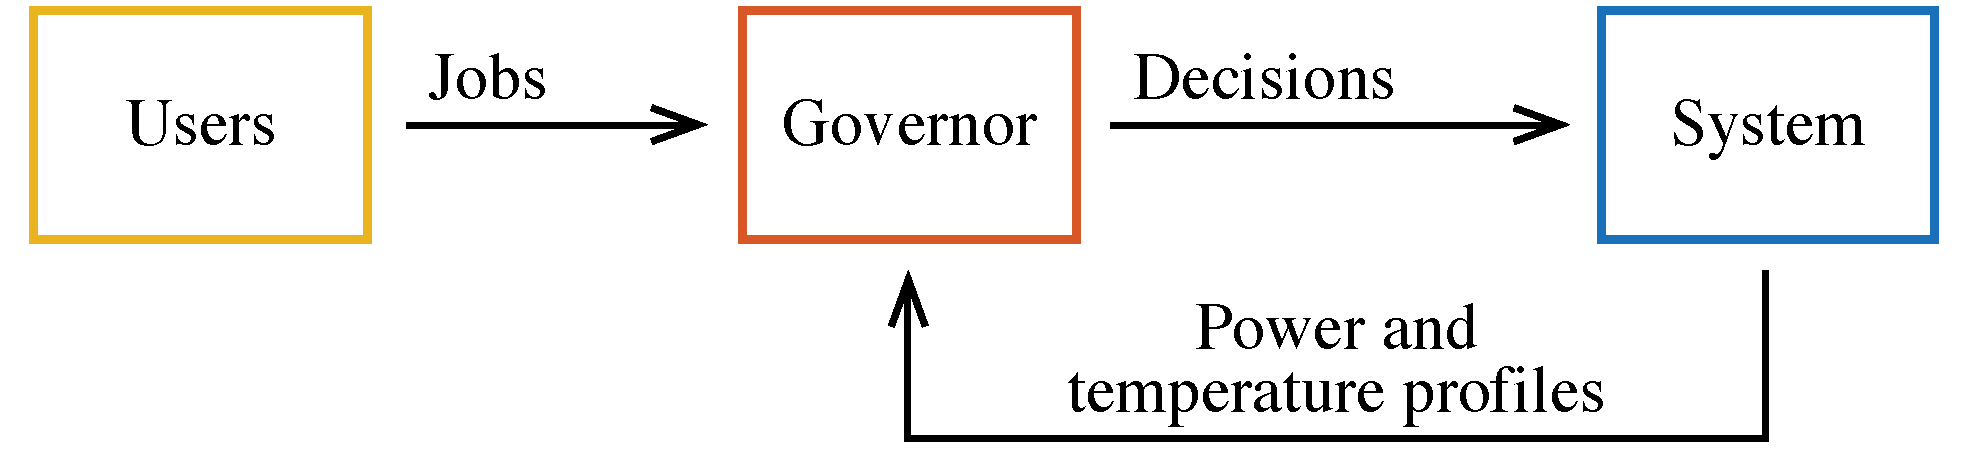
\includegraphics[width=1.0\columnwidth]{include/assets/figures/usage.pdf}
  \caption{A usage example with a feedback loop.}
  \flab{usage}
\end{figure}

A usage example with a feedback loop is given in \fref{usage}. Our methodology
revolves about the box in the middle and provides the boxes to the sides.
